101. На рисунке изображена развёртка игрального кубика. Сумма цифр на любых двух противоположных гранях равна 7. Какой может быть наибольшая разность цифр на закрашенных гранях? Напоминаем, что на всех гранях стоят разные цифры от 1 до 6.
\begin{center}
\begin{figure}[ht!]
\center{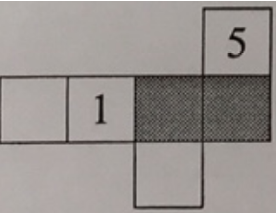
\includegraphics[scale=0.35]{17.png}}
\end{figure}
\end{center}
